\chapter{Zásuvný modul}
\label{4-plugin}

V~této kapitole je popsán samotný zásuvný modul. Pro~názornost a~srozumitelnost jsou zde uvedeny důležité části kódu a~diagramy znázorňující složitější algoritmy. Všechny snímky obrazovky byly pořízeny ve stylu grafického uživatelského prostředí \textit{GTK+}.

Během~vývoje zásuvného modulu bylo čerpáno z~literatury zabývající se programem QGIS \citep{pyqgis_book}~\citep{qgis_book}, programovacím jazykem Python \citep{dive_into_python} \citep{python3_oop_book} a modulem PyQt \citep{pyqt_book}.

\section{Instalace}
\label{instalace}

Zásuvný modul není součástí oficiálního repozitáře QGIS, přesto ho lze nainstalovat stejným způsobem jako~jiné pluginy. Stačí do~programu QGIS přidat repozitář organizace GeoForAll Lab\footnote{http://geomatics.fsv.cvut.cz/research/geoforall/}. Nejprve je tedy nutné otevřít okno s~repozitáři \textit{Zásuvné moduly $\rightarrow$ Spravovat a~instalovat zásuvné moduly $\rightarrow$ Nastavení} (viz obr.~\ref{fig:pridani_repozitare}) a~zde pomocí tlačítka \textit{Přidat...} doplnit repozitář GeoForAll Lab dostupný na~adrese \url{http://geo.fsv.cvut.cz/geoforall/qgis-plugins.xml} (viz obr.~\ref{fig:pridani_repozitare_geoforall_lab}). Zásuvný modul se řadí mezi experimentální, proto je zapotřebí aktivovat volbu \textit{Zobrazit také experimentální zásuvné moduly}, viz obr.~\ref{fig:pridani_repozitare}. Poté už stačí do~vyhledávacího pole zadat \textit{PU Plugin} a~zásuvný modul pro~pozemkové úpravy nainstalovat (viz obr.~\ref{fig:instalace_puplugin}).

	\begin{figure}[H]
		\centering
		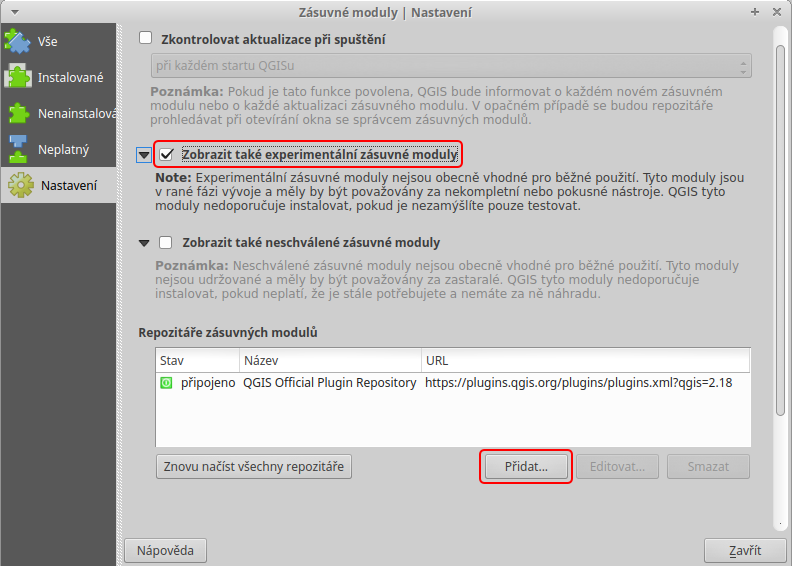
\includegraphics[width=.7\textwidth]{./pictures/pridani_repozitare.png}
		\caption[Přidání repozitáře]{Přidání repozitáře}
		\label{fig:pridani_repozitare}
 	\end{figure}
 	
	\begin{figure}[H]
		\centering
		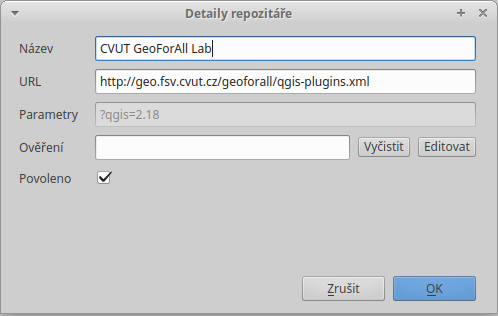
\includegraphics[width=.5\textwidth]{./pictures/pridani_repozitare-geoforall_lab.png}
		\caption[Přidání repozitáře GeoForAll Lab]{Přidání repozitáře GeoForAll Lab}
		\label{fig:pridani_repozitare_geoforall_lab}
 	\end{figure}

	\begin{figure}[H]
		\centering
		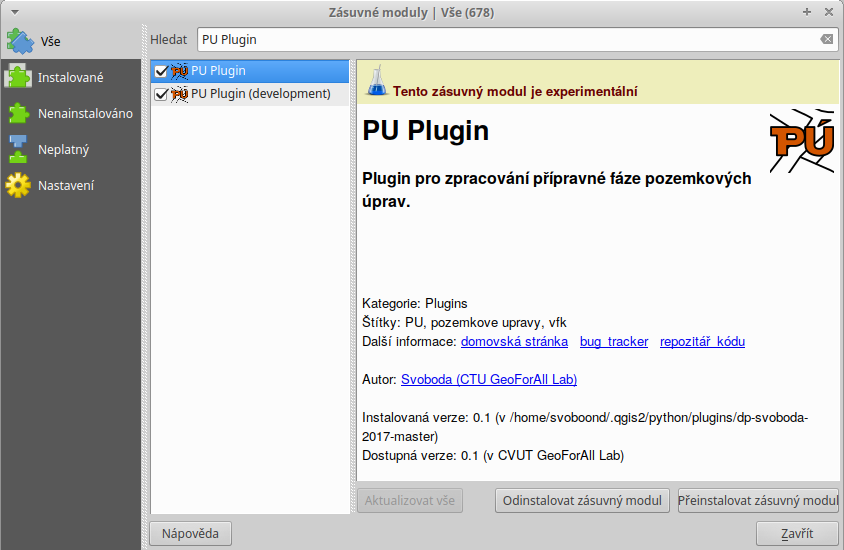
\includegraphics[width=.6\textwidth]{./pictures/instalace_puplugin.png}
		\caption[Instalace zásuvného modulu]{Instalace zásuvného modulu}
		\label{fig:instalace_puplugin}
 	\end{figure}

Když je plugin nainstalován, objeví se v~liště zásuvných modulů jeho ikona (viz obr.~\ref{fig:ikona_puplugin}). Okno zásuvného modulu je možné vyvolat poklepáním na~jeho ikonu nebo volbou \textit{Zásuvné moduly $\rightarrow$ PU Plugin $\rightarrow$ PU Plugin}.

	\begin{figure}[H]
		\centering
		
\includegraphics[width=.1\textwidth]{./pictures/puplugin.png}
		\caption[Ikona zásuvného modulu]{Ikona zásuvného modulu}
		\label{fig:ikona_puplugin}
 	\end{figure}

\section{Grafické uživatelské rozhraní}
\label{gui}

Grafické uživatelské rozhraní zásuvného modulu je reprezentováno jedním oknem (viz obr. \ref{fig:main_gui}), které je možné ukotvit do samotného programu QGIS. Protože zásuvný modul se řídí podle~legislativy české republiky a~používá výměnný formát katastru nemovitostí, je grafické uživatelské rozhraní v~českém jazyce.

	\begin{figure}[H]
		\centering
		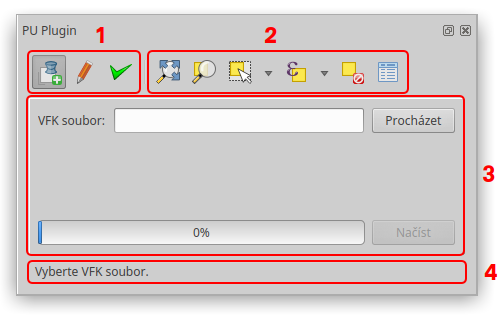
\includegraphics[width=.55\textwidth]{./pictures/main_gui.png}
		\caption[Grafické uživatelské rozhraní zásuvného modulu]{Grafické uživatelské rozhraní zásuvného modulu}
		\label{fig:main_gui}
 	\end{figure}

\begin{description}
	\item[Prvek 1:] Skupina tří ikon pro přepínání mezi záložkami:
	\begin{itemize}[leftmargin=1.5cm, noitemsep]
		\item \img{./pictures/loadvfk.png} \textit{Načtení VFK souboru}
		\item \img{./pictures/edit.png} \textit{Editace}
		\item \img{./pictures/checkanalysis.png} \textit{Kontroly a analýzy}
 	\end{itemize}
 	
	\item[Prvek 2:] Skupina nástrojů, které jsou propojené se standardními nástroji programu QGIS. Pokud tedy uživatel například aktivuje nástroj pro~výběr prvků polygonem v~okně zásuvného modulu, automaticky se aktivuje stejný nástroj v~panelu QGISu a~naopak.
	\begin{itemize}[leftmargin=1.5cm, noitemsep]
		\item \img{./pictures/zoom_full.png} \textit{Přiblížit na rozměry okna}
		\item \img{./pictures/zoom_to_selected.png} \textit{Přiblížit na výběr}
		\item tlačítko interaktivního výběru prvků z mapového okna
		\begin{itemize}[leftmargin=1.5cm, noitemsep]
			\item \img{./pictures/select_rectangle.png} \textit{Vybrat prvky oblastí nebo jednoklikem}
			\item \img{./pictures/select_polygon.png} \textit{Vybrat prvky polygonem}
			\item \img{./pictures/select_freehand.png} \textit{Vybrat prvky kreslením od ruky}
			\item \img{./pictures/select_radius.png} \textit{Vybrat prvky poloměrem}
 		\end{itemize}
		\item tlačítko výběru prvků
		\begin{itemize}[leftmargin=1.5cm, noitemsep]
			\item \img{./pictures/select_expression.png} \textit{Vybrat pomocí vzorce...}
			\item \img{./pictures/select_value.png} \textit{Vybrat prvky hodnotou...}
			\item \img{./pictures/select_all.png} \textit{Vybrat všechny prvky}
			\item \img{./pictures/invert_selection.png} \textit{Převrátit výběr prvků}
 		\end{itemize}
		\item \img{./pictures/deselect.png} \textit{Zrušit výběr prvků ve všech vrstvách}
		\item \img{./pictures/open_table.png} \textit{Otevřít atributovou tabulku}
 	\end{itemize}
	\item[Prvek 3:] Okna záložek zobrazující se v~závislosti na~tom, která ze~tří ikon záložek (prvkek~1) je aktivní.
	\item[Prvek 4:] Stavový řádek, ve~kterém se ukazují zprávy pro~uživatele.
\end{description}

\section{Komunikace s uživatelem}
\label{komunikace}

Zásuvný modul komunikuje s uživatelem třemi způsoby:

\begin{enumerate}[leftmargin=1.5cm, noitemsep]
	\item \underline{Stavový řádek} (viz prvek~4 obr.~\ref{fig:main_gui}) představuje nejčastější způsob zobrazování zpráv zásuvného modulu. Pokud  uživatel neví jak postupovat, zde s~největší pravděpodobností najde potřebné informace. Běžné zprávy mají černou barvu písma, důležíté zprávy se~zobrazují červeně (viz obr.~\ref{fig:dulezita_zprava}).
	
	\begin{figure}[H]
		\centering
		
\includegraphics[width=.23\textwidth]{./pictures/statusbar-red_message.png}
		\caption[Důležitá zpráva ve stavovém řádku]{Důležitá zpráva ve stavovém řádku}
		\label{fig:dulezita_zprava}
 	\end{figure}	

	\item \underline{Pole zpráv} je standardní způsob komunikace mezi programem QGIS a uživatelem. Zobrazuje pole v horní části mapového okna, které může být nastaveno tak, že po určité době samo zmizí, nebo vyžaduje zavření uživatelem. Zprávy mají čtyři urovně zobrazení, viz tab. \ref{tab:urovne_pole_zprav}.

\begin{table}[H]
    \begin{tabular}{|l|l|}
        \hline
         úroveň & český popis \\
        \hline
        \hline
         INFO & informační zpráva \\ \hline
         WARNING & zpráva upozornění \\ \hline
         CRITICAL & kritická zpráva \\ \hline
         SUCCESS & zpráva úspěchu \\
         \hline
    \end{tabular}
    \centering
    \caption[Úrovně zobrazení pole zpráv]{Úrovně zobrazení pole zpráv (zdroj:~\citep{qgis_api})}
    \label{tab:urovne_pole_zprav}
\end{table}

Zásuvný modul využívá této komunikace pouze pro zobrazení významných zpráv, které by neměly být uživatelem opomenuty (viz obr. \ref{fig:zprava_pole_zprav}).

	\begin{figure}[H]
		\centering
		
\includegraphics[width=.7\textwidth]{./pictures/message_bar-message.png}
		\caption[Zpráva upozornění v poli zpráv]{Zpráva upozornění v poli zpráv}
		\label{fig:zprava_pole_zprav}
 	\end{figure}

	\item \underline{Logování} je posledním prostředkem pro~předávání informací, který zásuvný modul používá. Informace v~anglickém jazyce, zejména chybové hlášky, zapisuje do vlastní záložky s~názvem \textit{PU Plugin} (viz obr. \ref{fig:logovaci_panel}). Panel logovacích zpráv lze zobrazit kliknutím na~ikonu \img{./pictures/log.png} v~pravém dolním rohu QGISu.

	\begin{figure}[H]
		\centering
		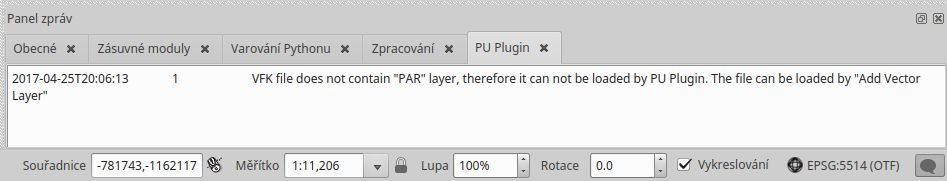
\includegraphics[width=1.0\textwidth]{./pictures/log_panel.png}
		\caption[Panel logovacích zpráv]{Panel logovacích zpráv}
		\label{fig:logovaci_panel}
 	\end{figure}

\end{enumerate}

\newpage

\section{Načtení VFK souboru}
\label{nacteni_vfk}

Prvním krokem při prácí se zásuvným modulem je načtení \zk{VFK} souboru. Právě k tomuto účelu slouží záložka, která se po nainstalování nebo spuštění pluginu zobrazuje.

\subsection{Grafické uživatelské rozhraní}
\label{nacteni_vfk_gui}

	\begin{figure}[H]
		\centering
		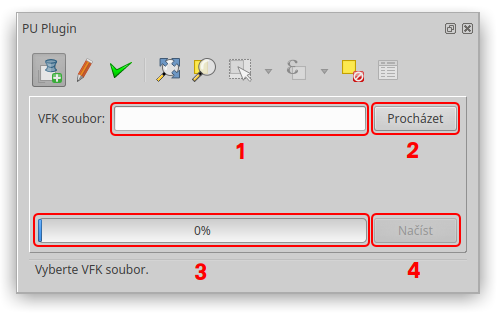
\includegraphics[width=.55\textwidth]{./pictures/nacteni_vfk_gui.png}
		\caption[Grafické uživatelské rozhraní záložky \textit{Načtení VFK souboru}]{Grafické uživatelské rozhraní záložky \textit{Načtení VFK souboru}}
		\label{fig:nacteni_vfk_gui}
 	\end{figure}

\begin{description}
	\item[Prvek 1:] Textové pole pro cestu k \zk{VFK} souboru.
	\item[Prvek 2:] Tlačítko pro zobrazení dialogového okna pro procházení adresářů. Filtruje soubory s příponou \textit{*.vfk}, pamatuje si poslední použitou cestu.
	\item[Prvek 3:] Indikátor průběhu načítání \zk{VFK} souboru.
	\item[Prvek 4:] Tlačítko pro načítání \zk{VFK} souboru. Aktivuje se pouze v~případě, že textové pole (prvek 1) obsahuje cestu k~existujícímu \zk{VFK} souboru.
\end{description}

\subsection{Postup}
\label{postup_nacteni_vfk}

Nejprve uživatel zvolí, který \zk{VFK} soubor chce načíst. K~dispozici jsou dva způsoby. Buď poklepá na~tlačítko \textit{Procházet} (prvek~2 na obr.~\ref{fig:nacteni_vfk_gui}), vybere požadovaný soubor a~cesta k~souboru se automaticky zapíše do~textového pole (prvek~1 na obr.~\ref{fig:nacteni_vfk_gui}), nebo zkopíruje cestu k~\zk{VFK} souboru přímo do~zmíněného textové pole. V~momentě, kdy se v~textovém poli nachází cesta k~validnímu \zk{VFK} souboru, se aktivuje tlačítko pro~načítání (prvek~4 na obr.~\ref{fig:nacteni_vfk_gui}) a~je možné zahájit import. O~průběhu načítání je uživatel informován indikátorem průběhu (prvek~3 na obr.~\ref{fig:main_gui}) a zprávami ve~stavovém řádku (prvek~4 na obr.~\ref{fig:main_gui}).

\subsection{Algoritmus}
\label{nacteni_vfk_algoritmus}

Algoritmus pro náčítání \zk{VFK} souborů patří mezi komplikovanější části zásuvného modulu a je klíčový pro správný chod navazujících procesů, proto je mu zde věnována zvýšená pozornost.

První verze tohoto algoritmu byla inspirována \zk{VFK} Pluginem\footnote{\detokenize{http://freegis.fsv.cvut.cz/gwiki/VFK_/_QGIS_plugin}}, ale během vývoje bylo nezbytné algoritmus mnohokrát upravovat a ve výsledku se dosti liší.

Pro čtení \zk{VFK} souborů používá QGIS knihovnu GDAL (viz kapitola č.~\ref{podklady}), konkrétně se jedná o \zk{VFK} Driver\footnote{\detokenize{http://www.gdal.org/drv_vfk.html}}. Ten funguje tak, že při prvním čtení souboru vytvoří ve stejném adresáři, ve kterém se nachází čtený \zk{VFK} soubor, SQLite databázi a do ní naimportuje všechna data. Pří dalším čtení se již databáze nevytváří, proto je čtení mnohonásobně rychlejší, viz tab.~\ref{tab:nacteni_vfk_driver}. 

\begin{table}[H]
    \begin{tabular}{|l|l|}
        \hline
         načtení & čas [s] \\
        \hline
        \hline
         první & 6.516 \\ \hline
         opakované & 0.160 \\
         \hline
    \end{tabular}
    \centering
    \caption[Porovnání rychlosti načtení VFK Driverem]{Porovnání rychlosti načtení VFK Driverem}
    \label{tab:nacteni_vfk_driver}
\end{table}

\zk{VFK} Driver ovšem umožňuje otevřít \zk{VFK} soubor pouze v~režimu čtení a to je pro~potřeby zpracování pozemkových úprav nedostatečné.

Pro takové případy je knihovna GDAL vybavena SQLite Driverem\footnote{\detokenize{http://gdal.org/drv_sqlite.html}}, který nabízí možnost zápisu do SQLite databáze. Aby byl SQLite driver schopen rozpoznat a přečíst geometrii, musí databáze obsahovat tabulky \textit{\detokenize{geometry_columns}} a~\textit{\detokenize{spatial_ref_sys}}. V~tabulce \textit{\detokenize{geometry_columns}} je uveden seznam tabulek, které mají geometrii, společně s~údaji jako název sloupce s~geometrií, typ geometrie, souřadnicový systém a~další, viz tab. \ref{tab:geometry_columns}. Údaje o souřadnicovém systému odkazují na~tabulku \textit{\detokenize{spatial_ref_sys}}, ve~které jsou souřadnicové systémy definovány. Seznam sloupců tabulky \textit{\detokenize{spatial_ref_sys}} a~jejich datové typy popisuje tab. \ref{tab:spatial_ref_sys}. 

\begin{table}[H]
    \begin{tabular}{|l|l|}
        \hline
         název sloupce & datový typ \\
        \hline
        \hline
         \detokenize{F_TABLE_NAME} & varchar unique \\ \hline
         \detokenize{F_GEOMETRY_COLUMN} & varchar \\ \hline
         \detokenize{GEOMETRY_TYPE} & integer \\ \hline
         \detokenize{COORD_DIMENSION} & integer \\ \hline
         \detokenize{SRID} & integer \\ \hline
         \detokenize{GEOMETRY_FORMAT} & varchar \\
         \hline
    \end{tabular}
    \centering
    \caption[Sloupce tabulky \textit{geometry\textunderscore columns}]{Sloupce tabulky \textit{geometry\textunderscore columns}}
    \label{tab:geometry_columns}
\end{table}

\begin{table}[H]
    \begin{tabular}{|l|l|}
        \hline
         název sloupce & datový typ \\
        \hline
        \hline
         \detokenize{SRID} & integer unique \\ \hline
         \detokenize{AUTH_NAME} & text \\ \hline
         \detokenize{AUTH_SRID} & text \\ \hline
         \detokenize{SRTEXT} & text \\
         \hline
    \end{tabular}
    \centering
    \caption[Sloupce tabulky \textit{spatial\textunderscore ref\textunderscore sys}]{Sloupce tabulky \textit{spatial\textunderscore ref\textunderscore sys}}
    \label{tab:spatial_ref_sys}
\end{table}

%% TODO - pridat odkaz na prilohu
Během prvních experimentů s daty souboru \zk{VFK} bylo zjištěno, že OGR poskytovatel programu QGIS při změně atributových hodnot nepoužíval transakce. V~důsledku toho trvalo uložení změn extrémně dlouho. Tato chyba byla nahlášena vývojářům systému QGIS, ti ji opravili a od verze 2.18.5 poskytovatel OGR transakce využívá. Podrobněji se tomuto tématu věnuje příloha TODO. Algoritmus zásuvného modulu pro načítání \zk{VFK} souboru zmíněný problém zohledňuje. Ve verzi programu QGIS nižší než 2.18.5 naimportuje data to databáze SpatiaLite\footnote{SpatiaLite je extenze SQLite, která umožňuje ukládat geoprostorová data. Obsahuje také mnoho funkcí pro analýzu geoprostorových dat \citep{spatialite} \citep{wiki_spatialite}} a dále s~ní pracuje (viz~\ref{kontrola_verze_qgis}). Poskytovatel SpatiaLite programu QGIS totiž ukládá změny v~transakcích a~tudíž nemá problémy s~pomalým zápisem.

{\scriptsize
\begin{lstlisting}[style=python, caption={Kontrola verze programu QGIS}, captionpos=b, label=kontrola_verze_qgis, backgroundcolor = \color{light-gray},  numbers=left]
if QGis.QGIS_VERSION < '2.18.5':
    self.fixedSqliteDriver = False
else:
    self.fixedSqliteDriver = True
\end{lstlisting}}

\subsubsection{Popis algoritmu}
\label{popis_algoritmu_nacteni_vfk}

Algoritmus načtení \zk{VFK} souboru funguje následovně.

Pokud v adresáři, ve kterém se nachází vstupní \zk{VFK} soubor, neexistuje databáze SQLite se stejným názvem, vytvoří se pomocí \zk{VFK} Driveru knihovny GDAL (viz~\ref{vytvoreni_db_vfk_driver}).

{\scriptsize
\begin{lstlisting}[style=python, caption={Vytvoření SQLite databáze pomocí VFK Driveru}, captionpos=b, label=vytvoreni_db_vfk_driver, backgroundcolor = \color{light-gray},  numbers=left]
QgsApplication.registerOgrDrivers()

vfkDriver = ogr.GetDriverByName('VFK')
vfkDataSource = vfkDriver.Open(filePath)
\end{lstlisting}}

Poté algoritmus zkontroluje, zda je v~databázi tabulka parcel (\zk{PAR}). Celý plugin pracuje téměř výhradně právě s~touto tabulkou, proto když ji databáze neobsahuje, algoritmus se ukončí. Uživatele na tento problém upozorní zprávy ve~stavovém řádku, poli zpráv i~logovací záložce (viz sekce~\ref{komunikace}). Následuje tvorba geometrie pro~tabulky \zk{PAR}, \zk{SPOL} a \zk{SOBR}.

V~dalším kroku se otevře databázové připojení. Databázovým dotazem se zkontroluje přítomnost tabulek \textit{\detokenize{geometry_columns}} a~\textit{\detokenize{spatial_ref_sys}}. Pokud to je nutné, pomocí SQL dávky se obě tabulky vytvoří a~nahrají se do nich potřebné údaje. Při editaci a~navazujících kontrolách a~analýzách zásuvný modul do tabulky parcel zapisuje vlastní data, proto je zapotřebí přidat vlastní sloupce. Dotazem se zjistí, jestli již v databázi existují, pokud ne, další SQL dávka zajistí jejich vytvoření. Seznam přidaných sloupců a jejich datové typy se nachází v~tab.~\ref{tab:pridane_sloupce_par}.

\begin{table}[H]
    \begin{tabular}{|l|l|}
        \hline
         název sloupce & datový typ \\
        \hline
        \hline
         \detokenize{PU_KMENOVE_CISLO_PAR} & integer \\ \hline
         \detokenize{PU_PODDELENI_CISLA_PAR} & integer \\ \hline
         \detokenize{PU_VYMERA_PARCELY} & integer \\ \hline
         \detokenize{PU_VYMERA_PARCELY_ABS_ROZDIL} & integer \\ \hline
         \detokenize{PU_VYMERA_PARCELY_MEZNI_ODCHYLKA} & integer \\ \hline
         \detokenize{PU_VYMERA_PARCELY_MAX_KODCHB_KOD} & integer \\ \hline
         \detokenize{PU_KATEGORIE} & integer \\ \hline
         \detokenize{PU_VZDALENOST} & integer \\ \hline
         \detokenize{PU_CENA} & real \\ \hline
         \detokenize{PU_BPEJ_BPEJCENA_VYMERA_CENA} & text \\ \hline
         \detokenize{PU_MERITKO_PODKLADU} & integer \\
         \hline
    \end{tabular}
    \centering
    \caption[Přidané sloupce do tabulky PAR]{Přidané sloupce do tabulky \zk{PAR}}
    \label{tab:pridane_sloupce_par}
\end{table}

Když je proces nahrávání spuštěn ve verzi programu nižší než 2.18.5, všechna data databáze SQLite se naimportují do databáze SpatiaLite.

Nakonec se tabulka parcel v závislosti na verzi QGISu pomocí SQLite (viz \ref{vytvoreni_vrstvy_parcel_pomoci_sqlite}) nebo SpatiaLite Driveru nahraje do~programu QGIS jako platná vrstva.

Načtení \zk{VFK} souboru je spuštěno v samostatném vlákně. Pro přehlednost celý popsaný proces ilustruje diagram na obr. \ref{fig:diagram_nacitani_vfk}.

{\scriptsize
\begin{lstlisting}[style=python, caption={Vytvoření vrstvy parcel pomocí SQLite Driveru}, captionpos=b, label=vytvoreni_vrstvy_parcel_pomoci_sqlite, backgroundcolor = \color{light-gray},  numbers=left]
blacklistedDriver = ogr.GetDriverByName('VFK')
blacklistedDriver.Deregister()

composedURI = dbPath + '|layername=PAR'
layer = QgsVectorLayer(composedURI, layerName, 'ogr')
	
blacklistedDriver.Register()
\end{lstlisting}}

	\begin{figure}[H]
		\centering
		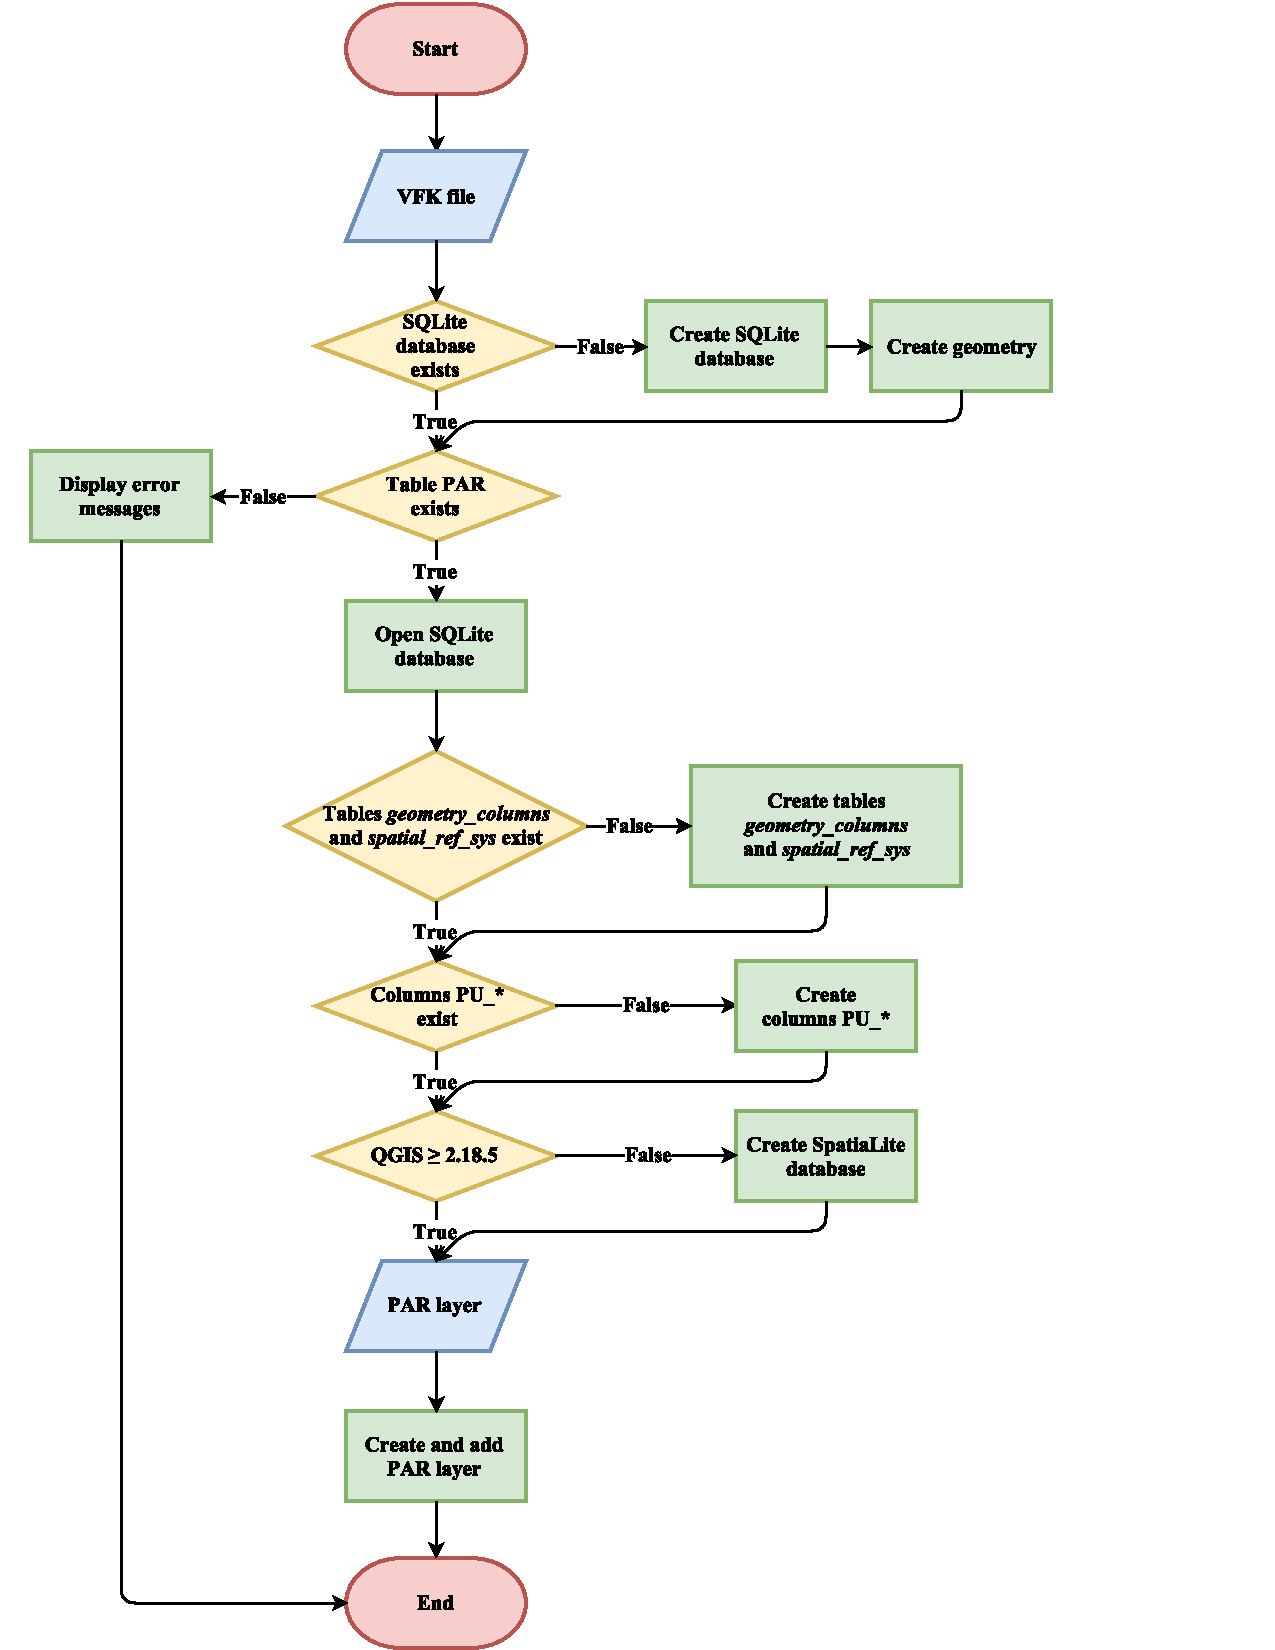
\includegraphics[width=1.2\textwidth]{./pictures/nacitani_vfk_souboru.pdf}
		\caption[Diagram algoritmu pro načítání VFK souboru]{Diagram algoritmu pro načítání VFK souboru}
		\label{fig:diagram_nacitani_vfk}
 	\end{figure}

\subsection{Symbologie vrstvy PAR}
\label{symbologie_par}

Symbologie nahrané vrstvy parcel je dána podle předem připraveného QML souboru, ve~kterém jsou definovány barvy podle druhů pozemků. V~tabulce parcel je informace o~druhu pozemku uvedena ve~sloupci \detokenize{DRUPOZ_KOD} (viz tab.~\ref{tab:par_sloupce}), kódy druhů pozemku s~názvy se nachází v tab.~\ref{tab:druhy_pozemku}. Při~větším přiblížení se zobrazí i~parcelní čísla. Ukázka symbolgie vrstvy parcel je k~nahlednutí na~obr.~\ref{fig:symbologie_par}.

\begin{table}[H]
    \begin{tabular}{|l|l|}
        \hline
         kód & název \\
        \hline
        \hline
          2 & orná půda \\ \hline
          3 & chmelnice \\ \hline          
          4 & vinice \\ \hline
          5 & zahrada \\ \hline
          6 & ovocný sad \\ \hline
          7 & trvalý travní porost \\ \hline
          10 & lesní pozemek \\ \hline
          11 & vodní plocha \\ \hline
          13 & zastavěná plocha a nádvoří \\ \hline
          14 & ostatní plocha \\
         \hline
    \end{tabular}
    \centering
    \caption[Druhy pozemků]{Druhy pozemků (zdroj \citep{vyhlaska_357})}
    \label{tab:druhy_pozemku}
\end{table}

	\begin{figure}[H]
		\centering
		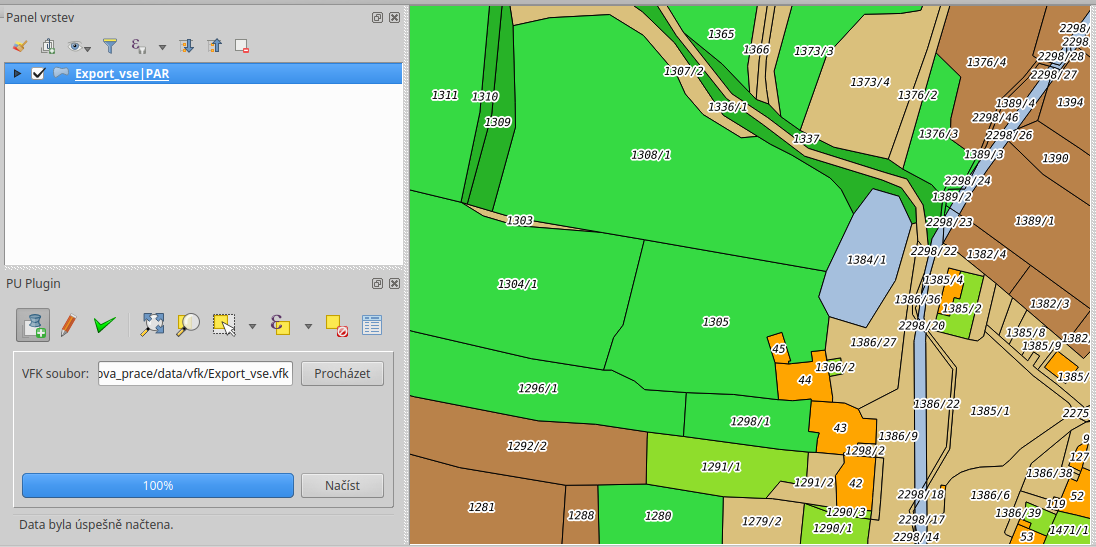
\includegraphics[width=1.0\textwidth]{./pictures/symbologie_par.png}
		\caption[Symbologie vrstvy parcel]{Symbologie vrstvy parcel}
		\label{fig:symbologie_par}
 	\end{figure}

\subsection{Atributová tabulka vrstvy PAR}
\label{tabulka_par}

Tabulka parcel sama o sobě obsahuje mnoho sloupců. Společně se sloupci, které přidává zásuvný modul, se atributová tabulka stává nepřehlednou, proto plugin všechny nepotřebné sloupce v atributové tabulce skrývá. Kvůli větší srozumitelnost pro uživatele navíc přidává sloupcům aliasy, viz tab. \ref{tab:viditelne_sloupce_aliasy_par}.

\begin{table}[H]
    \begin{tabular}{|l|l|}
        \hline
         název sloupce & alias \\
        \hline
        \hline
          \detokenize{KMENOVE_CISLO_PAR} & KMENOVE C. (PUV.) \\ \hline
          \detokenize{PU_PODDELENI_CISLA_PAR} & PODDELENI C. (EDI.) \\ \hline
          \detokenize{PODDELENI_CISLA_PAR} & PODDELENI C. (PUV.) \\ \hline
          \detokenize{PU_KMENOVE_CISLO_PAR} & KMENOVE C. (EDI.) \\ \hline
          \detokenize{PU_KATEGORIE} & KATEGORIE \\ \hline
          \detokenize{VYMERA_PARCELY} & VYMERA (SPI) \\ \hline
          \detokenize{PU_VYMERA_PARCELY} & VYMERA (SGI) \\ \hline
          \begin{tabular}{@{}l@{}} \detokenize{PU_VYMERA_PARCELY} \\ \detokenize{_ABS_ROZDIL} \end{tabular} & ROZ. VYMER \\ \hline
          \begin{tabular}{@{}l@{}} \detokenize{PU_VYMERA_PARCELY} \\ \detokenize{_MEZNI_ODCHYLKA} \end{tabular} & MEZ. ODCH. ROZ. VYMER \\ \hline
          \detokenize{PU_VZDALENOST} & VZDALENOST \\ \hline
          \detokenize{PU_CENA} & CELK. CENA \\ \hline
          \begin{tabular}{@{}l@{}} \detokenize{PU_BPEJ} \\ \detokenize{_BPEJCENA_VYMERA_CENA} \end{tabular} & \begin{tabular}{@{}l@{}} BPEJ KOD-CENA ZA M2 \\ -VYMERA-CENA \end{tabular} \\ \hline
          \detokenize{PU_MERITKO_PODKLADU} & MERITKO PODKL. \\
         \hline
    \end{tabular}
    \centering
    \caption[Viditelné sloupce a~aliasy vrstvy parcel]{Viditelné sloupce a~aliasy vrstvy parcel}
    \label{tab:viditelne_sloupce_aliasy_par}
\end{table}

\newpage

\section{Editace}
\label{editace}

Když je vrstva parcel úspěšně nahrána do programu QGIS, lze začít s editací. Záložka \textit{Editace} slouží k úpravě geometrie a zařazení parcel do kategorií (viz část \ref{predmet_pu}).

\subsection{Grafické uživatelské rozhraní}
\label{editace_gui}

	\begin{figure}[H]
		\centering
		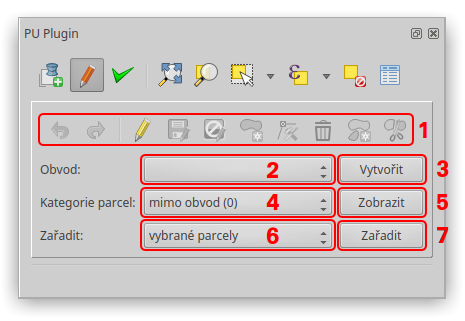
\includegraphics[width=.55\textwidth]{./pictures/editace_gui.png}
		\caption[Grafické uživatelské rozhraní záložky \textit{Editace}]{Grafické uživatelské rozhraní záložky \textit{Editace}}
		\label{fig:editace_gui}
 	\end{figure}

\begin{description}
	\item[Prvek 1:] Skupina nástrojů pro editaci propojených se~standardními nástroji programu QGIS.
	\begin{itemize}[leftmargin=1.5cm, noitemsep]
		\item \img{./pictures/undo.png} \textit{Zpět}
		\item \img{./pictures/redo.png} \textit{Znovu}
		\item \img{./pictures/toggle_editing.png} \textit{Přepnout editaci}
		\item \img{./pictures/save_edits.png} \textit{Uložit změny vrstvy}
		\item \img{./pictures/cancel_edits.png} \textit{Zrušit pro vybrané vrstvy}
		\item \textit{Přidat prvek}
		\begin{itemize}[leftmargin=1.5cm, noitemsep]
			\item \img{./pictures/add_line.png} liniový prvek
			\item \img{./pictures/add_point.png} bodový prvek
			\item \img{./pictures/add_polygon.png} polygonový prvek
 		\end{itemize}
		\item \img{./pictures/node_tool.png} \textit{Nástroj uzlů}
		\item \img{./pictures/delete_selected.png} \textit{Vymazat vybrané}
		\item \img{./pictures/add_part.png} \textit{Přidat část}
		\item \img{./pictures/split_feature.png} \textit{Rozdělit objekt}
 	\end{itemize}
	\item[Prvek 2:] Rozbalovací menu s~aktuálně načtenými polygonovými vrstvami.
	\item[Prvek 3:] Tlačítko pro~zobrazení dialogového okna pro~uložení vrstvy obvodu. Filtruje soubory s~příponou \textit{*.pu.shp} , pamatuje si poslední použitou cestu.
	\item[Prvek 4:] Rozbalovací menu s~kategoriemi parcel (viz část \ref{predmet_pu}). Na výběr jsou tyto kategorie, číslo v závorce udává hodnotu, kterou zásuvný modul pro kategorii používá:
	\begin{itemize}[leftmargin=1.5cm, noitemsep]
		\item \textit{mimo obvod (0)}
		\item \textit{v obvodu - neřešené (1)}
		\item \textit{v obvodu - řešené (2)}
		\item \textit{bez kategorie}
	\end{itemize}
	\item[Prvek 5:] Tlačítko pro zobrazení (vybrání) parcel v~aktuálně zvolené kategorii.
	\item[Prvek 6:] Rozbalovací menu s~variantami zařazení parcel. K dispozici jsou dvě možnosti:
	\begin{itemize}[leftmargin=1.5cm, noitemsep]
		\item \textit{vybrané parcely} - zařadí vybrané parcely do aktuálně zvolené kategorie.
		\item \textit{obvodem} - zařadí všechny parcely do kategorií na základě obvodu.
	\end{itemize}
	\item[Prvek 7:] Tlačítko pro provedení zařazení.
\end{description}

\subsection{Postup}
\label{postup_editace}

Zásuvný modul pracuje s aktivní vrstvou, tj. vrstva vybraná v panelu vrstev, který se ve výchozím nastavení nachází na levé straně okna.

Vrstva parcel je otevřená pomocí SQLite Driveru\footnote{Ve verzi programu QGIS nižší než~2.18.5 je vrstva otevřená Spatialite Driverem, viz \ref{nacteni_vfk_algoritmus}.}, takže~jí je možné editovat. K~tomuto účelu slouží sada standardních nástrojů v~horní části pluginu (viz prvek~1 na~obr.~\ref{fig:editace_gui}).

Nejdůležitější funkcionalitou této záložky je ovšem zařazení parcel do~kategorií. Aby bylo na~první pohled zřejmé, ve~které kategorii jsou jednotlivé parcely zařazeny, používá zásuvný modul tzv.~vrstvu obvodu. Jedná se o~samostatnou vrstvu ve~formátu \textit{shapefile}, která není součástí SQLite databáze, ale~ukládá se na~disk. Adresář a~název této vrstvy může uživatel specifikovat pomocí tlačítka \textit{Vytvořit}\footnote{Pro~odlišení tohoto souboru od~jiných dat uživatele, se ke~zvolenému názvu přidá přípona \textit{*.pu.shp}} (viz prvek~3 na obr. \ref{fig:editace_gui}). Po poklepání na zmíněné tlačítko se otevře dialogové okno, kde uživatel zvolí umístění vrstvy obvodu. Z aktivní vrstvy, která musí být \zk{VFK}, se vytvoří vrstva obvodu, zásuvný modul ji načte a vybere v rozbalovacím menu (viz prvek~2 na obr. \ref{fig:editace_gui}).

Pokud cesta k vrstvě obvodu není uživatelem definována (rozbalovací menu je prázdné), nebo je v rozbalovací menu vybrána vrstva, která nebyla vytvořena zásuvným modulem a tudíž neobsahuje potřebné sloupce, plugin automaticky vytvoří vrstvu obvodu ve stejném adresáři, ve kterém se nachází aktivní \zk{VFK} vrstva.

Funkce pro vytvoření obvodu je volána v momentě, kdy je pro vrstvu \zk{VFK} uložena změna geometrie\footnote{Signál s názvem \textit{committedGeometriesChanges}.}, uložena změna, při které došlo k vymazání prvku\footnote{Signál s názvem \textit{committedFeaturesRemoved}.}, nebo je pomocí tlačítka \textit{Zařadit} (prvek 7 na obr. \ref{fig:editace_gui}) provedeno zařazení parcel.

Zásuvný modul nabízí dvě varianty zařazení parcel (viz prvek 6 na obr. \ref{fig:editace_gui}). První a zcela jistě více používanou možností je volba \textit{vybrané parcely}, která provede zařazení vybraných parcel do zvolené kategorie (viz prvek~4 na obr. \ref{fig:editace_gui}).

Druhý způsob nazvaný \textit{obvodem} rozřadí všechny parcely ve~\zk{VFK} vrstvě do~kategorií. Jako podklad použije aktuálně vybranou vrstvu obvodu (viz prvek~2 na obr. \ref{fig:editace_gui}). Tato varianta pracuje pouze s obvody, které vytvořil zásuvný modul pro pozemkové úpravy. Pro~zařazení do~kategorie musí být parcela kompletně uvnitř geometrie příslušného prvku obvodu\footnote{Plugin používá nástroj \textit{Select by location} s~geometrickým predikátem \textit{within}.}.

Pro kontrolu nabízí zásuvný modul tlačítko \textit{Zobrazit} (viz prvek 5 na~obr. \ref{fig:editace_gui}), které vybere, a~tím pádem zvýrazní, prvky v~kategorii (viz \ref{vyber_prvku_v_kategorii}).

{\scriptsize
\begin{lstlisting}[style=python, caption={Výběr prvků v kategorii parcel}, captionpos=b, label=vyber_prvku_v_kategorii, backgroundcolor = \color{light-gray},  numbers=left]
expression = QgsExpression("\"PU_KATEGORIE\" = {}".format(value))
features = layer.getFeatures(QgsFeatureRequest(expression))

ids = [feature.id() for feature in features]
layer.selectByIds(ids)
\end{lstlisting}}

%% TODO - doplnit referenci
Při~zpracování pozemkových úprav se stává, že je potřeba zdigitalizovat parcelu na~základě podkladové mapy. Právě proto přidává zásuvný modul do~tabulky parcel sloupec \detokenize{PU_MERITKO_PODKLADU} (alias MERITKO PODKL.). Pokud tedy uživatel vytvoří novou parcelu, nebo~pomocí nástroje \textit{Přidat část} doplní popisné údaje o geometrii, měl by vyplnit měřítko podkladů. Tento údaj používá \textit{kontrola - výměra nad mezní odchylkou} (viz část TODO).

\subsection{Symbologie vrstvy obvodu}
\label{symbologie_obvod}

Symbologie vrstvy obvodu se stejně jako u~vrstvy parcel řídí podle QML souboru. Kvůli~výraznosti byla zvolena červená barva, popisky obsahují pouze číslo kategorie. Symbologie vrstvy obvodu je znázorněna na~obr. \ref{fig:symbologie_obvod}, kde je také vidět použití tlačítka \textit{Zobrazit}.

	\begin{figure}[H]
		\centering
		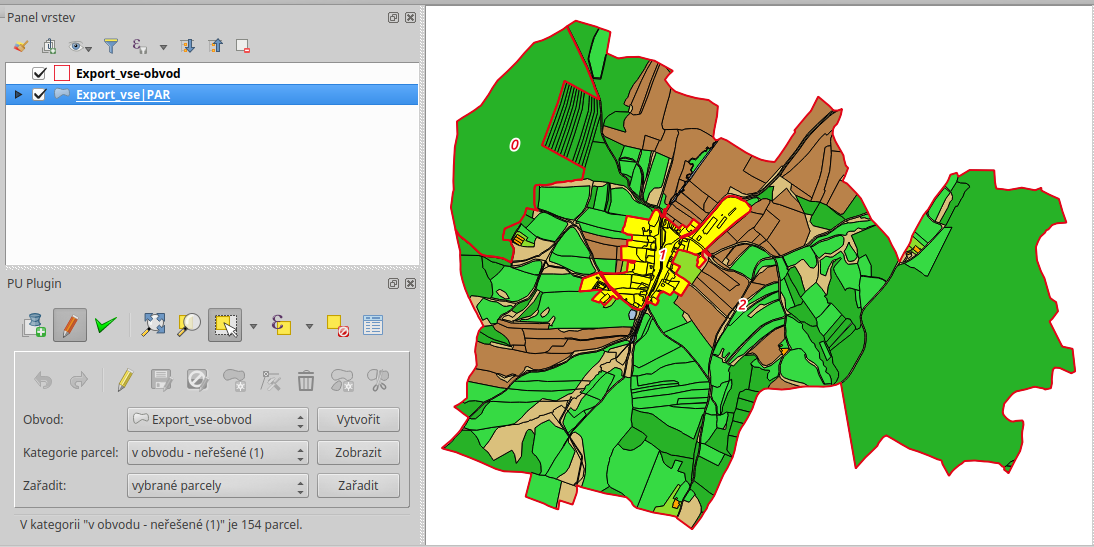
\includegraphics[width=1.0\textwidth]{./pictures/symbologie_obvod.png}
		\caption[Grafické uživatelské rozhraní záložky \textit{Editace}]{Grafické uživatelské rozhraní záložky \textit{Editace}}
		\label{fig:symbologie_obvod}
 	\end{figure}

\subsection{Atributová tabulka vrstvy obvodu}
\label{tabulka_obvod}

Vrstva obvodu se vytváří z vrstvy parcel, ovšem pouze informace o~kategorii je pro~obvod relevantní. Z~toho důvodu je viditelný pouze sloupec \detokenize{PU_KATEGORIE}, viz tab.~\ref{tab:viditelne_sloupce_aliasy_obvod}.

\begin{table}[H]
    \begin{tabular}{|l|l|}
        \hline
         název sloupce & alias \\
        \hline
        \hline
          \detokenize{PU_KATEGORIE} & KATEGORIE \\
         \hline
    \end{tabular}
    \centering
    \caption[Viditelné sloupce a~aliasy vrstvy obvodu]{Viditelné sloupce a~aliasy vrstvy obvodu}
    \label{tab:viditelne_sloupce_aliasy_obvod}
\end{table}

\newpage

\section{Kontroly a analýzy}
\label{kontroly_analyzy}

Poslední záložka zásuvného modulu nabízí možnost zkontrolovat data, zejména soulad mezi~\zk{SPI} a~\zk{SGI}, a~provést analýzy nezbytné pro~sestavení nárokových listů.

\subsection{Grafické uživatelské rozhraní}
\label{ca_gui}

	\begin{figure}[H]
		\centering
		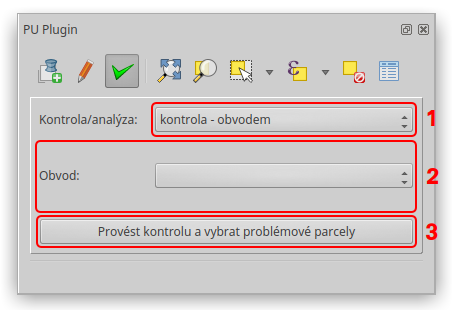
\includegraphics[width=.55\textwidth]{./pictures/ca_gui.png}
		\caption[Grafické uživatelské rozhraní záložky \textit{Kontroly a analýzy}]{Grafické uživatelské rozhraní záložky \textit{Kontroly a analýzy}}
		\label{fig:ca_gui}
 	\end{figure}

\begin{description}
	\item[Prvek 1:] Rozbalovací menu pro přepínání mezi kontrolami a analýzami.
	\item[Prvek 2:] Okna kontrol a analýz zobrazující se v~závislosti na~tom, která položka rozbalovacího menu (prvek~1) je vybrána.
	\item[Prvek 3:] Tlačítko pro provedení kontroly či analýzy. Jeho text je pro kontroly a~analýzy rozdílný.
\end{description}

\subsection{Postup}
\label{postup_ca}

Práce v~záložce \textit{Kontroly a~analýzy} je velmi jednoduchá a~intuitivní. V~rozbalovacím menu uživatel zvolí kontrolu či~analýzu, důsledkem čehož se změní okno kontroly (prvek~2 na~obr.~\ref{fig:ca_gui}). Některé kontroly nevyžadují žádné nastavení, u~analýz a~jiných kontrol se od~uživatele očekává určitá interakce, bez~které není možné pokračovat. Když je vše potřebné zadané, lze kontrolu či~analýzu spustit. O~výsledku je uživatel informován pomocí zpráv ve~stavovém řádku.

\subsection{Kontroly}
\label{kontroly}

\subsubsection{Kontrola - obvodem}
\label{kontrola_obvodem}

Kontrola obvodem provádí výběr parcel, které nejsou kompletně uvnitř vrstvy obvodu\footnote{Použit je nástroj \textit{Select by location} s~geometrickým predikátem \textit{within} a~poté je zavolána funkce pro~převrácení výběru prvků.}.

Pokud uživatel pracuje od~začátku pouze s~jednou vrstvou obvodu, měl by být výsledek této kontroly stejný jako při~zvolení kategorie \textit{bez kategorie} (viz prvek~4 na obr.~\ref{fig:editace_gui}) a~provedení výběru prvků v~kategorii pomocí tlačítka \textit{Zobrazit} (viz prvek 5 na obr. \ref{fig:editace_gui}). Lišit se tyto dvě metody budou v~momentě, kdy si uživatel nahraje vrstvu obvodu, kterou vytvořil s jinou vrstvou parcel. Jinými slovy tato kontrola používá geometrii vrstvy obvodu a tlačítko \textit{Zobrazit} v záložce \textit{Editace} vybírá parcely na základě údajů uložených v~atributové tabulce.

Jediným potřebným vstupem je zmiňovaná vrstva obvodu v~rozbalovacím menu (viz obr.~\ref{fig:kontrola_obvodem_gui}), které je propojené s~menu vrstvy obvodu v~záložce \textit{Editace}.

	\begin{figure}[H]
		\centering
		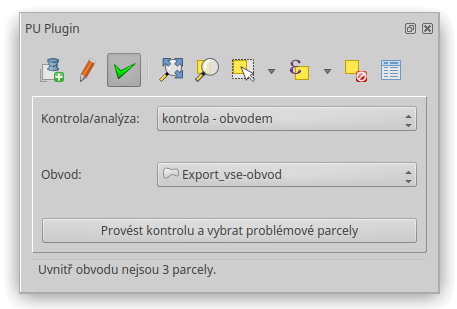
\includegraphics[width=.55\textwidth]{./pictures/kontrola-obvodem.png}
		\caption[Grafické uživatelské rozhraní kontroly \textit{obvodem}]{Grafické uživatelské rozhraní kontroly \textit{obvodem}}
		\label{fig:kontrola_obvodem_gui}
 	\end{figure}

\subsubsection{Kontrola - není v SPI}
\label{kontrola_neni_v_spi}

Jak vyplývá z~názvu, kontrola \textit{není v SPI} slouží k~zobrazení parcel, které nejsou v~souboru popisných informací. Pro výběr používá sloupec \detokenize{KMENOVE_CISLO_PAR}, neboť patří mezi povinně vyplněné \citep{struktura_vfk}. Pokud má parcela tento sloupec prázdný, znamená to, že se jedná o~nově vytvořenu parcelu. Provedení kontroly \textit{není v SPI} nevyžaduje žádné nastavení, jedinou podmínkou je aktivní vrstva parcel.

\subsubsection{Kontrola - není v mapě}
\label{kontrola_neni_v_mape}

Ani~pro~spuštění kontroly \textit{není v mapě} uživatel nemusí cokoli zadávat, stačí mít aktivní vrstvu \zk{PAR}. Po~dokončení jsou vybrány parcely, které mají nulovou geometrii a~tudíž se nezobrazují v~mapovém okně\footnote{Vybrány jsou též parcely s~nevalidní geometrií.}.

\subsubsection{Kontrola - výměra nad mezní odchylkou}
\label{kontrola_vymera}

Kontrola \textit{výměra nad~mezní odchylkou} ověřuje, zda~rozdíl mezi výměrou dle~\zk{SPI} a~výměrou vypočtenou z~\zk{SGI} nepřekračuje mezní odchylku. Ta je stanovena katastrální vyhláškou \citep{vyhlaska_357} a~závisí na~kódu kvality nejméně přesně určeného lomového bodu na~hranici parcely, viz tab.~\ref{tab:odchylky_vymer}. Jestliže je parcela digitalizovaná, kód kvality podrobných bodů se určí podle~měřítka podkladové mapy, viz tab.~\ref{tab:kody_kvality_digit}.

	\begin{figure}[H]
		\centering
		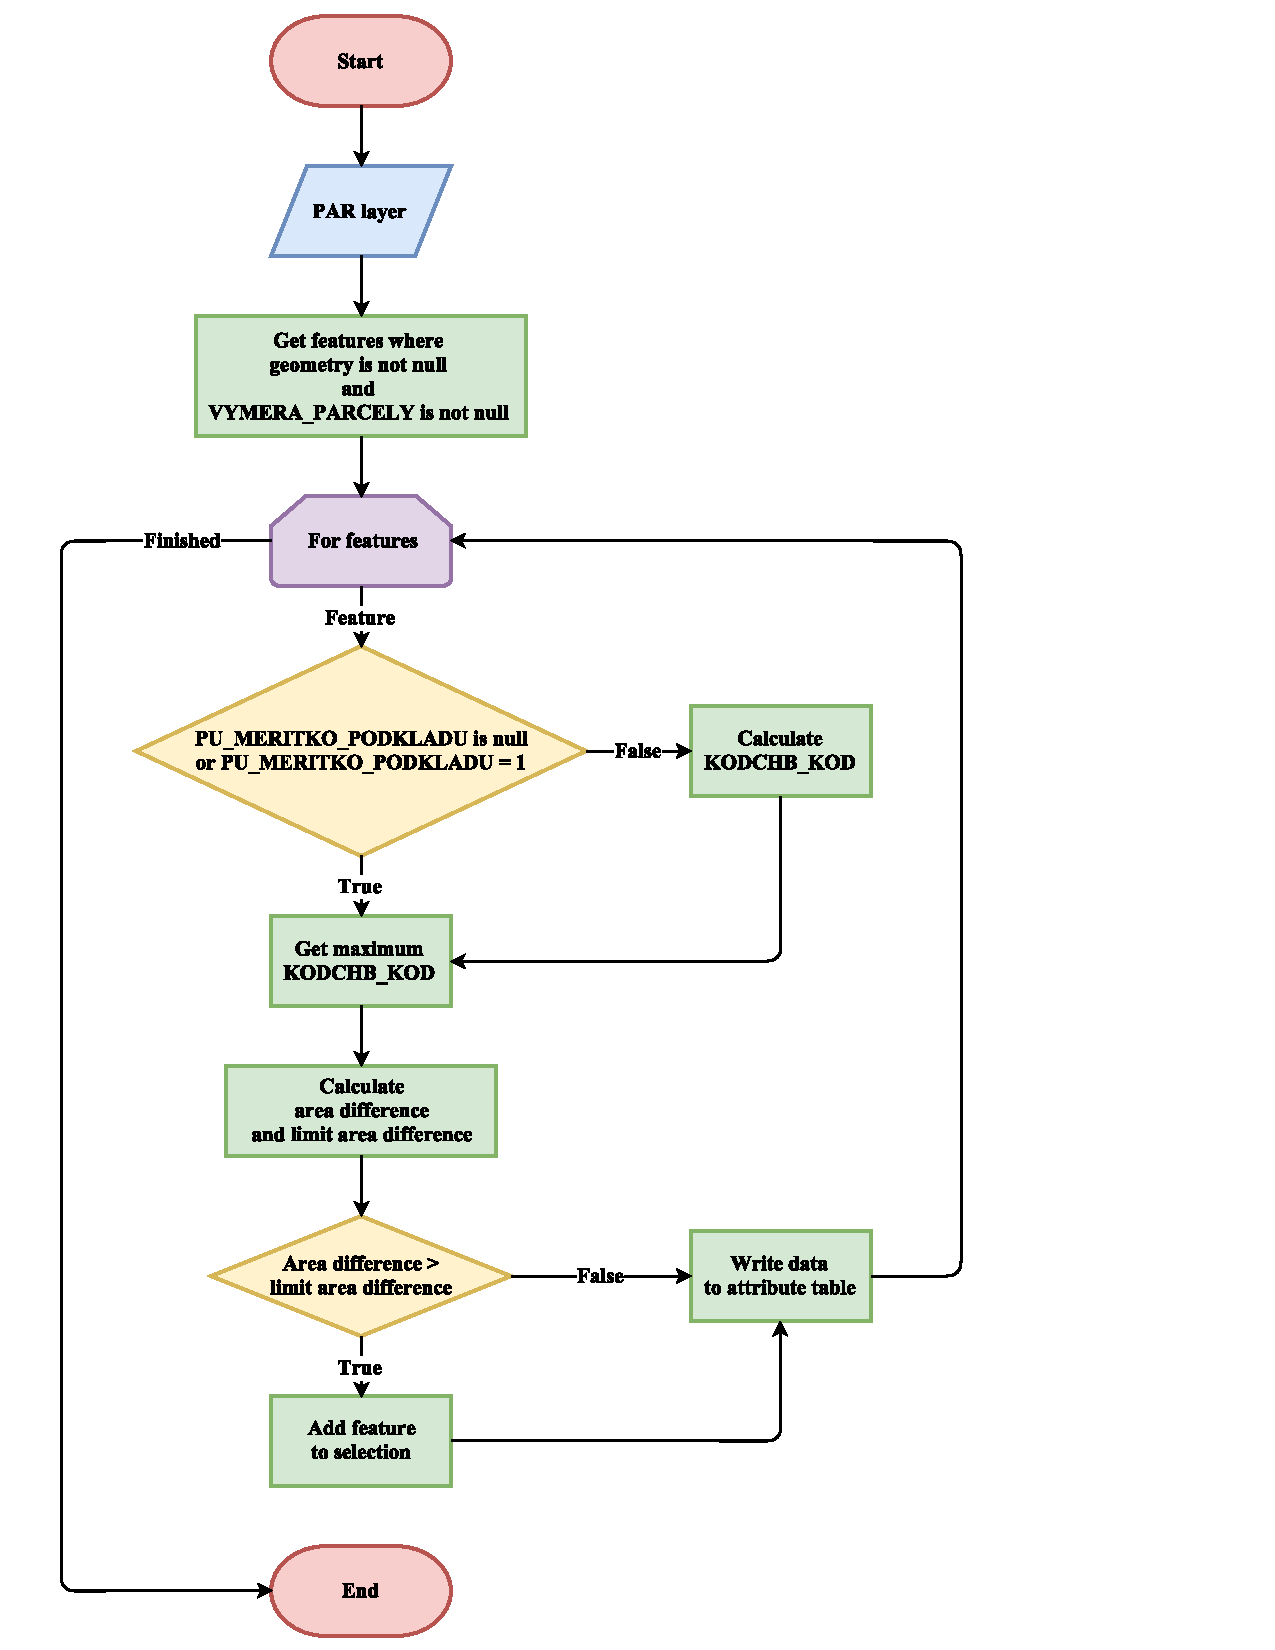
\includegraphics[width=1.2\textwidth]{./pictures/vymera.pdf}
		\caption[Diagram algoritmu kontroly \textit{výměra nad mezní odchylkou}]{Diagram algoritmu kontroly \textit{výměra nad mezní odchylkou}}
		\label{fig:diagram_vymera}
 	\end{figure}

%%BPEJ je zjednodusene - viz 9.8 http://www.spucr.cz/frontend/webroot/uploads/files/2015/12/metodickynavodkprovadenipozemkovychuprav1327.pdf